\documentclass[10pt,a4paper,spanish]{report}

\usepackage[spanish]{babel}
\usepackage[utf8]{inputenc}
\usepackage{amsmath, amsthm}
\usepackage{amsfonts, amssymb, latexsym}
\usepackage{enumerate}
% \usepackage[official]{eurosym}
\usepackage{graphicx}
\usepackage[usenames, dvipsnames]{color}
\usepackage{colortbl}
\usepackage{multirow}
\usepackage{fancyhdr}
\usepackage[all]{xy}
\usepackage{minted}
\usepackage{tikz}
\usepackage{pgfplots}
\usepackage{cancel}
\pgfplotsset{compat=1.5}

\headsep 3mm

\usepackage[bookmarks=true,
            bookmarksnumbered=false, % true means bookmarks in
                                     % left window are numbered
            bookmarksopen=false,     % true means only level 1
                                     % are displayed.
            colorlinks=true,
            linkcolor=webblue]{hyperref}
\definecolor{webgreen}{rgb}{0, 0.5, 0} % less intense green
\definecolor{webblue}{rgb}{0, 0, 0.5}  % less intense blue
\definecolor{webred}{rgb}{0.5, 0, 0}   % less intense red

\newcommand{\HRule}{\rule{\linewidth}{0.5mm}} % regla horizontal para  el titulo

\pagestyle{fancy}
%con esto nos aseguramos de que las cabeceras de capítulo y de sección vayan en minúsculas

\renewcommand{\chaptermark}[1]{%
      \markboth{#1}{}}
\renewcommand{\sectionmark}[1]{%
      \markright{\thesection\ #1}}
\fancyhf{} %borra cabecera y pie actuales
\fancyhead[LE,RO]{{\bfseries\leftmark}}
\fancyhead[LO]{\bfseries Marta Gómez}
\fancyfoot[C]{\thepage{}}
\renewcommand{\headrulewidth}{0.5pt}
\renewcommand{\footrulewidth}{0pt}
\addtolength{\headheight}{0.5pt} %espacio para la raya
\fancypagestyle{plain}{%
      \fancyhead{} %elimina cabeceras en páginas "plain"
      \renewcommand{\headrulewidth}{0pt} %así como la raya
}

% %%%%% Para cambiar el tipo de letra en el título de la sección %%%%%%%%%%%
% \usepackage{sectsty}
% \chapterfont{\fontfamily{frc}\selectfont}
% \sectionfont{\fontfamily{pag}\selectfont}
% \subsectionfont{\fontfamily{pag}\selectfont}
% \subsubsectionfont{\fontfamily{pag}\selectfont}

\newmintedfile[mycplusplus]{c++}{
    linenos,
    numbersep=5pt,
    gobble=0,
    frame=lines,
    framesep=2mm,
    tabsize=3,
}

\newmintedfile[mypython]{python}{
    linenos,
    numbersep=5pt,
    gobble=0,
    frame=lines,
    framesep=2mm,
    tabsize=3,
}

\definecolor{amaranth}{rgb}{0.9, 0.17, 0.31}

\usepackage[sfdefault,light]{roboto}  %% Option 'sfdefault' only if the base font of the document is to be sans serif
\usepackage[T1]{fontenc}

\setlength{\parindent}{0pt}
\setlength{\parskip}{1ex plus 0.5ex minus 0.2ex}

\usepackage{titlesec}

% \titleformat{\chapter}{\normalfont\huge\center}{--- \thechapter ---}{20pt}{}

\titleformat
{\chapter} % command
[display] % shape
{\Huge\center\bfseries} % format
{--- \thechapter ---} % label
{0.5ex} % sep
{
    \rule{\textwidth}{1pt}
    \vspace{1ex}
    \centering
} % before-code
[
\vspace{-0.5ex}%
\rule{\textwidth}{0.3pt}
] % after-code

\newcommand*{\titleGM}{\begingroup % Create the command for including the title page in the document
\hbox{ % Horizontal box
\hspace*{0.2\textwidth} % Whitespace to the left of the title page
\rule{1pt}{\textheight} % Vertical line
\hspace*{0.05\textwidth} % Whitespace between the vertical line and title page text
\parbox[b]{0.75\textwidth}{ % Paragraph box which restricts text to less than the width of the page

{\noindent\Huge\bfseries Prácticas de \\[0.5\baselineskip] Algorítmica}\\[2\baselineskip] % Title
{\large \textit{Curso 2014/2015}}\\[4\baselineskip] % Tagline or further description
{\Large \textsc{Marta Gómez Macías}} % Author name

\vspace{0.5\textheight} % Whitespace between the title block and the publisher
{\noindent Universidad de Granada}\\[\baselineskip] % Publisher and logo
}}
\endgroup}


%Definimos autor y título
\title{\Huge Prácticas de \\ Algorítmica}
\author{Marta Gómez Macías}

\begin{document}
\thispagestyle{empty}
\titleGM

\tableofcontents

\chapter{\textcolor[rgb]{0.5,0.2,0.9}Eficiencia}
\section{\textcolor[rgb]{0.8,0,0.5}Enunciado}
{\Large Calcular la eficiencia en el caso promedio para el siguiente algoritmo:}

\begin{center}
\begin{minipage}{0.4\textwidth}
\usemintedstyle{monokai}
\definecolor{fondo}{rgb}{0.1,0.1,0.1}
\begin{minted}[linenos, frame=single, bgcolor=fondo]{c++}
i = 1;
while (i <= n) {
    if (a[i] >= a[n])
        a[n] = a[i];

    i *= 2;
}
\end{minted}
\end{minipage}
\end{center}

\section{\textcolor[rgb]{0.2,0.55,1}Solución}
En primer lugar, nos tenemos que preguntar cuántas veces se repite el bucle. En este caso el bucle sería equivalente a este otro: \mint{c++}|for (int i=1; i<=n; i=i*2)| al ir incrementándose la $i$ multiplicándose por dos en cada iteración hasta $n$, podemos decir que el bucle tendrá $\log_2 n$ iteraciones.

Para calcular el caso promedio, necesitamos calcular todos los casos posibles de ejecución que tiene el programa y hacer la media de todos. Empecemos por el mejor y peor caso.

En el mejor de los casos, la condición de la línea 3 ($a[i] \geq a[n]$) será falsa $\log_2 n$ veces y por tanto, no se ejecutará la sentencia del \verb*|if| ninguna vez. Por tanto, la eficiencia de nuestra función sería:

\begin{displaymath}
\underbrace{1}_{i=1} + \sum_{i=1}^{\log_2 n} (\underbrace{3}_{if} + \underbrace{2}_{i*=2} + \underbrace{1}_{while (i <= n)}) = 1 + \sum_{i=1}^{\log_2 n} 6 = 1 + 6 \cdot \sum_{i=1}^{\log_2 n} 1 = 1 + 6\log_2 n \in \Omega(\log_2 n)
\end{displaymath}

En el peor de los casos, pasará todo lo contrario: la condición de la línea 3 ($a[i] \geq a[n]$) será cierta $\log_2 n$ veces y por tanto, siempre se ejecutará la sentencia del \verb*|if|. Por tanto, la eficiencia de nuestra función sería:

\begin{displaymath}
\underbrace{1 + \sum_{i=1}^{\log_2 n} (3 + 2 + 1}_{\textrm{Lo que teníamos antes}} + \underbrace{3}_{a[n]=a[i]}) = 1 + \sum_{i=1}^{\log_2 n} 9 = 1 + 9 \cdot \sum_{i=1}^{\log_2 n} 1 = 1 + 9\log_2 n \in O(\log_2 n)
\end{displaymath}

Tenemos ya calculadas la eficiencia en el mejor y en el peor de los casos pero con sólo esos dos datos no podemos calcular aún la eficiencia en el caso promedio pues no tendríamos un resultado significativo. Para ello identificamos todos los casos que puede haber: desde el mejor, el \verb*|if| cierto en 0 ocasiones, hasta el peor, el \verb*|if| cierto en $\log_2 n$ ocasiones, pasando por 1, 2, 3, $\cdots$ ocasiones en las que son ciertas el \verb*|if|. Todos los casos son igual de probables (enfoque de máxima verosimilitud).

\begin{displaymath}
T(n) = \sum_{j=0}^{\log_2 n} Prob \bigg[a[i] \geq a[n] \textrm{ cierta en $j$ ocasiones, $0 \leq j \leq \log_2 n$} \bigg] \times
\end{displaymath}
\begin{displaymath}
t \bigg[ a[i] \geq a[n] \textrm{ falsa en $j$ ocasiones, $0 \leq j \leq \log_2 n$} \bigg] = 
\end{displaymath}
\begin{displaymath}
= \sum_{j=0}^{\log_2 n} \frac{1}{\log_2 (n+1)} \times \Bigg[ \underbrace{1}_{i=1} + \underbrace{\sum_{k=1}^{j}(1+3+3+2)}_{\textrm{$j$ ocasiones en las que el if es cierto}} + \underbrace{\sum_{k=j+1}^{\log_2 n} (1+3+2)}_{\textrm{$j$ ocasiones en las que el if es falso}} \Bigg] =
\end{displaymath}
\begin{displaymath}
= \sum_{j=0}^{\log_2 n} \frac{1}{\log_2 (n+1)} \times \Bigg[ 1 + 9j + 6(\log_2 (n-j)) \Bigg] = \sum_{j=0}^{\log_2 n} \frac{1}{\log_2 (n+1)} (6 \log_2 n + 3j + 1) =
\end{displaymath}
\begin{displaymath}
= \frac{1}{\log_2 (n+1)} \Bigg( 6 \log_2 n  \sum_{j=0}^{\log_2 n} 1  + 3 \sum_{j=0}^{\log_2 n} j + \sum_{j=0}^{\log_2 n} 1 \Bigg) = 
\end{displaymath}
\begin{displaymath}
= \frac{1}{\log_2 (n+1)} \Bigg( 6 \log_2 n \cdot \log_2 n + \frac{3\log_2 n}{2}\log_2 (n+1) + \log_2 n \Bigg) = 
\end{displaymath}
\begin{displaymath}
= \frac{6 \log_2^2 n + \frac{3\log_2 n}{2}\log_2 (n+1) + \log_2 n}{\log_2 (n+1)} = \frac{\cancel{\log_2 n} (6\log_2 n + \frac{3}{2}\log_2 (n+1) + 1)}{\cancel{\log_2 (n+1)}} \in \theta(\log_2 n)
\end{displaymath}

Y así concluimos que la eficiencia en el caso promedio es $\log_2 n$, tal y como se esperaba, pues la eficiencia del caso mejor y del peor también era $\log_2 n$ y, por tanto, también debía serlo la del caso promedio pues debe encontrarse entre el mejor y el peor caso.

\chapter{\textcolor[rgb]{0.9,0.3,0.35}Eficiencia en funciones recursivas}
\section{\textcolor[rgb]{0.9,0.3,0.35}Enunciado}
{\Large Calcular la eficiencia de la función recursiva representada por la siguiente ecuación:

\begin{equation*}
T(n) = \left\{
\begin{array}{rl}
1 & \text{si } n = 1,\\
3T(\frac{n}{2}) + n & \text{si } n > 1.
\end{array} \right.
\end{equation*}
}

\section{\textcolor[rgb]{0.2,0.55,1}Solución}
Nos quedamos con la parte que depende de $T$, es decir, el caso $n > 1$ y aplicamos un cambio de variable para transformar la ecuación en el tipo de ecuaciones con el que solemos trabajar:

\begin{displaymath}
n = 2^k \Longrightarrow k = \log_2 n \qquad\ T(2^k) = t_k
\end{displaymath}

Así, la ecuación nos queda de la siguiente forma:

\begin{displaymath}
T(2^k) = 3T(2^{k-1}) + 2^k
\end{displaymath}
\begin{displaymath}
t_k = 3t_{k-1} + 2^k
\end{displaymath}

Ahora que ya tenemos nuestra ecuación de modo más ``familiar'' para nosotros, pasamos a resolverla como cualquier otra ecuación:

\begin{center}
En primer lugar, pasamos todo lo que dependa de $t$ a un miembro:
\begin{displaymath}
t_k - 3t_{k-1} = 2^k
\end{displaymath}

Ahora obtenemos las raíces de la parte homogénea:
\begin{displaymath}
(x-3)=0
\end{displaymath}

Y las de la parte no homogénea. Para calcularlas debemos tener en cuenta la parte no homogénea es de la forma $b \cdot p(n)$ y las raíces, $(x-b)^{\textrm{grado de }p(n)+1}$

En este caso, al ser el polinomio $p(n)$ de grado $0$, las raíces de la parte no homogénea serían:
\begin{displaymath}
  (x-2)=0
\end{displaymath}

Por tanto nuestro polinomio característico sería:
\begin{displaymath}
t_k = c_1 3^k + c_2 2^k
\end{displaymath}

Pero esa no es nuestra solución final, pues está en función de $k$ y no en función de $n$. Debemos deshacer el cambio de variable:
\begin{displaymath}
T(n) = c_1 3^{\log_2 n} + c_2 2^{\log_2 n} = c_1 3^{\frac{\log_3 n}{\log_3 2}} + n \cdot c_2 =
\end{displaymath}

Tras conseguir cambiar el logaritmo de base, ahora debemos quitar la fracción que se ha quedado en el exponente:

\begin{displaymath}
= c_1 \cdot (3^{\log_3 n})^{\frac{1}{\log_3 2}} + c_2 \cdot n = c_1 \cdot n^{\frac{1}{\log_3 2}} + c_2 \cdot n = 
\end{displaymath}

Para  ello, volvemos a aplicar el cambio de base del logarimo:

\begin{displaymath}
= c_1 \cdot n^{\frac{1}{\frac{\log_2 2}{\log_2 3}}} + c_2 \cdot n = c_1 \cdot n^{\frac{1}{\frac{1}{\log_2 3}}} + c_2 \cdot n =
\end{displaymath}
\begin{displaymath}
= c_1 \cdot n^{\log_2 3} + c_2 \cdot n
\end{displaymath}
\end{center}

Tras obtener la ecuación, ahora debemos asegurarnos de que $c_1$ no es nulo ($c_1$ no puede ser negativo porque si no, obtendríamos tiempos de ejecución negativos) para poder afirmar que nuestro algoritmo es $O(n^{\log_2 3})$. Para ello, no podemos usar el caso base, pues no representa un tiempo de ejecución real porque éste depende de factores externos como el sistema operativo, la máquina, los tipos de datos... %pues no representa realmente ni al algoritmo ni al tiempo de ejecución, debido a que se va a aplicar cuando tengamos tamaños del problema muy grandes.

Entonces... ¿cómo comprobamos que $c_1$ no es nulo? Sustituyendo en la ecuación original:

\begin{center}
\begin{displaymath}
n = T(n) - 3T\Big(\frac{n}{2}\Big) = \underbrace{(\cancel{c_1 \cdot n^{\log_2 3}} + c_2 \cdot n)}_{T(n)} - \underbrace{3\Bigg(\cancel{c_1 \cdot \Big(\frac{n}{2}\Big)^{\log_2 3}} + c_2 \cdot \Big(\frac{n}{2}\Big)\Bigg)}_{3T(\frac{n}{2})}
\end{displaymath}

$c_1 \cdot n^{\log_2 3}$ y $3 \cdot \Bigg(c_1 \cdot \Big(\frac{n}{2}\Big)^{\log_2 3}\Bigg)$ se cancelan porque son el mismo número con signo contrario:

\begin{displaymath}
-3 c_1 \Big(\frac{n}{2}\Big)^{\log_2 3} = - c_1 n^{\log_2 3} \cdot \Big(3 \Big(\frac{1}{2}\Big)^{\log_2 3}\Big) = -c_1 \cdot n^{\log_2 3} \cdot \Big(\frac{3}{2 \log_2 3}\Big) = -c1 \cdot n^{\log_2 3} \cdot 1
\end{displaymath}

Por tanto, nos queda la siguiente ecuación:

\begin{displaymath}
n = c_2 \cdot n - 3 \cdot c_2 \cdot \frac{n}{2} = c_2 \cdot n \cdot \Big(1 - \frac{3}{2}\Big) =  \frac{-c_2 \cdot n}{2}
\end{displaymath}

Y despejando $c_2$, nos queda que $c_2 = -2$.
\end{center}

Por tanto, podemos confirmar que $c_1$ es positivo ya que si fuese nulo, el tiempo de ejecución sería negativo.

\chapter{\textcolor[rgb]{0.5,1,0.2}Divide y Vencerás}
\section{\textcolor[rgb]{0,0.2,1}Enunciado}
{\Large Implementa en primer lugar el método clásico de multiplicación de enteros largos. Después, implementa el método de Karatsuba y Ofman. Compara la eficiencia de ambos métodos.}

\section{\textcolor[rgb]{1,0.6,0}Solución}
\subsection{\textcolor[rgb]{1,0,0.6}Implementación del método clásico}
El algoritmo implementado hace lo siguiente:
\begin{enumerate}
  \item En primer lugar, guarda los dos números cada uno en un vector
  \item Después, implementa la multiplicación ``de toda la vida'' de dos números. Por ejemplo:

  \begin{center}
  \input{ej_mult.latex}
  \end{center}

  Para ello:
  \begin{enumerate}
    \item Añade ceros al principio de cada fila, para conseguir un desplazamiento.
    \item Multiplica cada elemento del segundo número por cada uno del primero, implementando los restos de cada multiplicación.
    \item Tras hacer todas las multiplicaciones, añade ceros al final de cada fila hasta completar el tamaño de la última.
    \item Suma las filas dos a dos hasta conseguir la solución:
    \begin{displaymath}
    (((filas[0]+filas[1])+filas[2])+\cdots+filas[n-1])
    \end{displaymath}
  \end{enumerate}
\end{enumerate}

La eficiencia de este algoritmo sería de $O(n^2)$ porque recorremos ambos vectores.

\mypython[label={MetodoClasico.py}]{multc.py}

\subsection{\textcolor[rgb]{0.7,0.2,0.4}Implementación del algoritmo de Karatsuba y Ofman}
El algoritmo implementado hace lo siguiente:
\begin{enumerate}
  \item Si los enteros que le pasamos son de una cifra, los multiplicamos directamente
  \item Si no, los dividimos de la siguiente forma:
  \begin{center}
  \input{explicacion_kyo.latex}
  \end{center}
  Procurando que ambos sean del mismo tamaño, es decir, que si uno es mayor que el otro, insertamos ceros no significativos hasta que ambos tengan el mismo tamaño.
  \item Los vamos dividiendo hasta conseguir enteros de una cifra que multiplicar.
  \item Una vez hecho esto, combinamos todas las soluciones parciales obtenidas con la siguiente fórmula:
  \begin{displaymath}
  u \cdot v = 10^{2 \cdot (\frac{n}{2})} \cdot w \cdot y + 10^{\frac{n}{2}} \cdot \Big[ (w-x) \cdot (z-y) + w \cdot y + x \cdot z \Big] + x \cdot z
  \end{displaymath}

  Es decir, dividimos nuestro problema en tres subproblemas:
  \begin{enumerate}[\color{amaranth}{$\heartsuit$}]
    \item $m_1 = w \cdot y$
    \item $m_2 = x \cdot z$
    \item $m_3 = (w-x) \cdot (z-y)$
  \end{enumerate}

  Así, reducimos el número de operaciones a $n^{1.59}$
\end{enumerate}

\mypython[label={karatsuba\_and\_ofman.py}]{multd.py}

\subsection{\textcolor[rgb]{0.51,0.28,0.47}Comparación del método clásico y del algoritmo Divide y Vencerás}
Cuando multiplicamos enteros \textit{\textcolor[rgb]{0.51,0.28,0.47}{no muy largos}}, la multiplicación clásica es más eficiente que la multiplicación divide y vencerás.

Por ejemplo, al multiplicar un entero de 10 cifras por sí mismo obtenemos un mejor tiempo con el método clásico (0.00048732757568359375 segundos frente a 0.0019004344940185547). En cambio, si ya multiplicamos un entero de 70 ya sí obtenemos una mejora en el divide y vencerás (0.019910812377929688 segundos frente a 0.015142202377319336):

\begin{center}
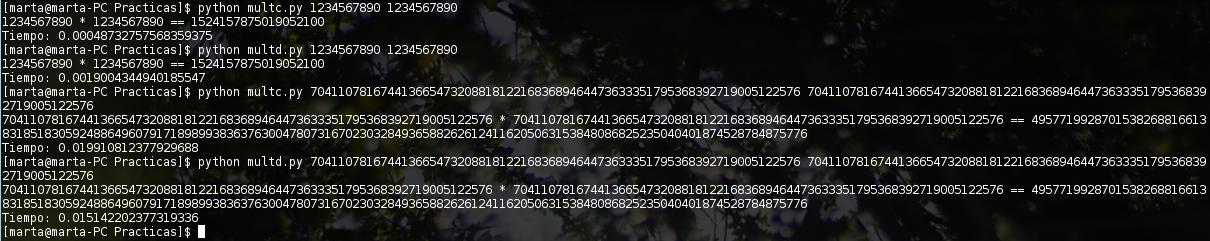
\includegraphics[width=1.2\textwidth]{comparacion_dyv1}
\end{center}

Cuanto mayor es el número, más se nota la diferencia, como se ve en esta foto en la que obtenemos un tiempo de 0.05 segundos con divide y vencerás y 0.2 con la multiplicación clásica:

\begin{center}
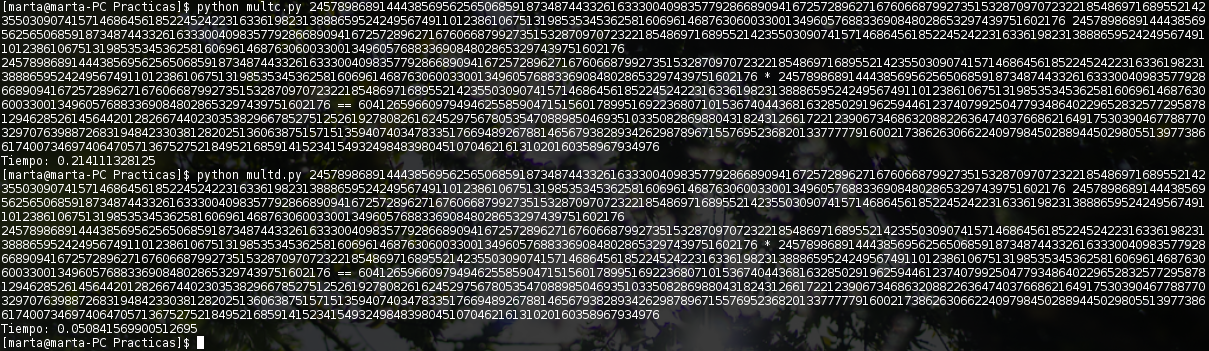
\includegraphics[width=1.2\textwidth]{comparacion_dyv2}
\end{center}


\chapter{\textcolor[rgb]{0.4,0.4,0.2}Algoritmos voraces}
\section{\textcolor[rgb]{0.5,1,1}Enunciado}
{\Large Implementa el problema de la mochila en C++ usando un algoritmo voraz. La función escogerá un objeto $obj1$ sobre otro, $obj2$ si se cumple la siguiente relación:
\begin{displaymath}
\frac{obj1.beneficio}{obj1.peso} > \frac{obj2.beneficio}{obj2.peso}
\end{displaymath}
}

\section{\textcolor[rgb]{0.8,1,0.2}Solución}
\subsection{\textcolor[rgb]{1,0.2,0.8}Implementación}
\mycplusplus[label={mochila.cpp}]{mochila.cpp}

\subsection{\textcolor[rgb]{0.5,0.2,1}Ejemplos de ejecución}
\begin{center}
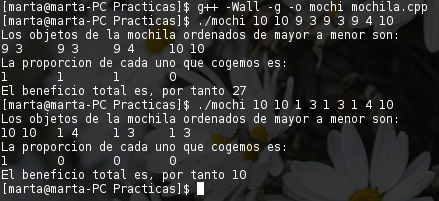
\includegraphics[width=0.7\textwidth]{voraces_ej}
\end{center}

\chapter{\textcolor[rgb]{0.2, 0.55, 0.2}Programación dinámica}
\section{\textcolor[rgb]{0.1,0.54,0.7}Enunciado}
{\Large Implementa el problema de la mochila en C++ usando programación dinámica.}

\section{\textcolor[rgb]{0.6,0.4,0.6}Solución}
El código lo que hace es ir rellenando una tabla de manera recursiva siguiendo la siguiente fórmula:

\begin{equation*}
Mochila(k,m) = 
\begin{cases}
0 & \text{si } k = 0 \text{ ó } m = 0,\\
-\infty & \text{si } k<0 \text{ ó } m<0\\
max\{Mochila(k-1,m), b_k + Mochila(k-1,m-p_k)\}
\end{cases} 
\end{equation*}

Así, empezaría rellenando la primera fila y la primera columna con ceros y a partir de ahí iría calculando el resto.

La implementación sería la siguiente:

\mycplusplus[label={mochila\_dinamica.cpp}]{mochila_dinamica.cpp}

\chapter{\textcolor[rgb]{1.0, 0.13, 0.32}Branch\&Bound}
\section{\textcolor[rgb]{0.13, 0.67, 0.8}Enunciado}
{\Large Implementa el problema de la mochila en C++ usando programación dinámica.}

\section{\textcolor[rgb]{1, 0.44, 0.37}Solución}
El código va generando un árbol binario a partir de los objetos de una lista que pasamos como parámetro del programa. Un ejemplo de ejecución sería el siguiente:

$pesomochi = 11$

$objetos(b, p) = \Big\{ [4,3]~[7,2]~[2,4]~[3,6] \Big\}$

El arbol generado sería el siguiente:

\input{arbol_ej.latex}

El código en cuestión, sería el siguiente:

\mycplusplus[label={mochila\_branchandbound.cpp}]{mochila_branchandbound.cpp}

\end{document}